\documentclass[11pt]{article}
\usepackage{report}

\title{Solid State Physics \\ Notes}
\author{Jesper Vesterberg (jeve0010@student.umu.se)}

\date{\today}

\begin{document}
\begin{titlepage}
  \maketitle
  \thispagestyle{fancy}
  \lhead{
    Department of physics\\
    Umeå Universitet
  }
  \rhead{\today}
  \begin{abstract}
		Collected notes of the whole course, base primarly on the course material (i.e.\ hook and halls book ``solid state physics'')
  \end{abstract}
	\cfoot{Solid State Physics}
\end{titlepage}
\lhead{\theauthor}
\rhead{\thetitle\\\today}
\cfoot{\thepage}


\section{Crystal Structure}
\subsection{Elementary Crystallography}
\subsubsection{The crystal lattice}
The crystal lattice is a way to describe crystal structures. We can take for example graphite as showed in figure~\ref{fig:graphite}. In order to create the lattice we take a point in the structure, lets call it $O$, then we need to find all identical positions within the structure.

\begin{figure}[H]
	\centering
	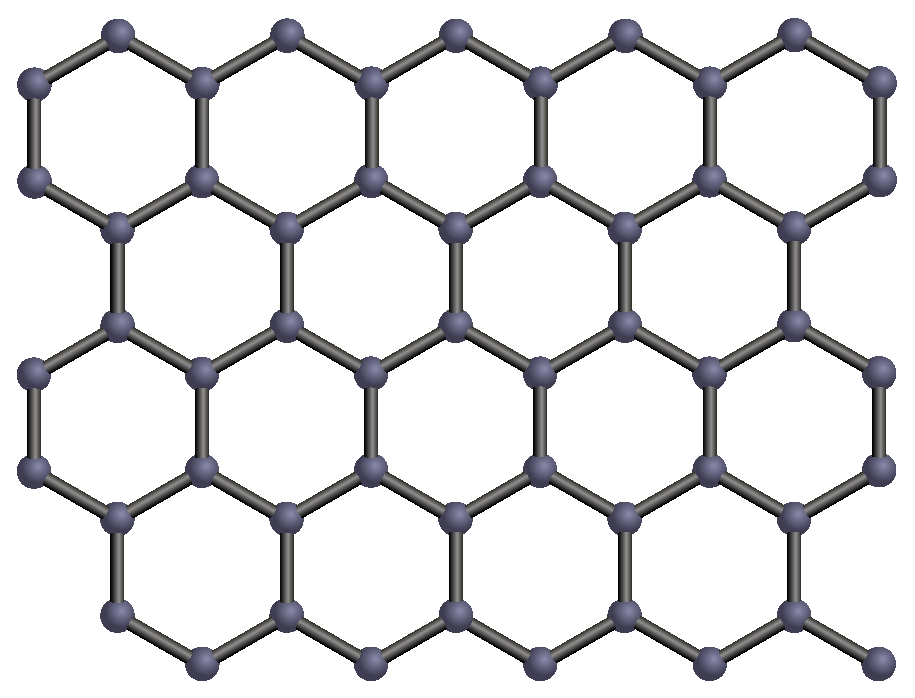
\includegraphics[width=0.8\textwidth]{graphite}
	\caption{Graphite lattice}
	\label{fig:graphite}
\end{figure}

\newpage
This choosing of $O$ and identification of identical position within the structure has been done in figure~\ref{fig:graphite-lattice}. Using this lattice which is highlighted in the dotted lines we see we have atoms on all lattice points except the atoms circled in yellow. This actually just fine, this is because we define all atoms related to lattice point through something called the basis, which we will look at in section~\ref{sec:basis}, this means that the crystal lattice do not have to coincide with any atom at all. Using the vectors $\mathbf{a}$ and $\mathbf{b}$ here we can define a vector which uniquely defines a point in the lattice relative $O$
\begin{equation}
	\mathbf{r}_{uv }= u\mathbf{a} + v\mathbf{v}
	\label{eq:crystal-lattice}
\end{equation}
All points defined through this equation are together called the \textbf{crystal lattice}. An important thing of this lattice is that it possesses \textbf{translational invariance}, which basically means that no matter from what lattice point you're looking at, the structure and environment looks precisely the same. For this to hold we need to presume that the lattice is practically infinite, which is something that is generally true. 

\begin{figure}[H]
	\centering
	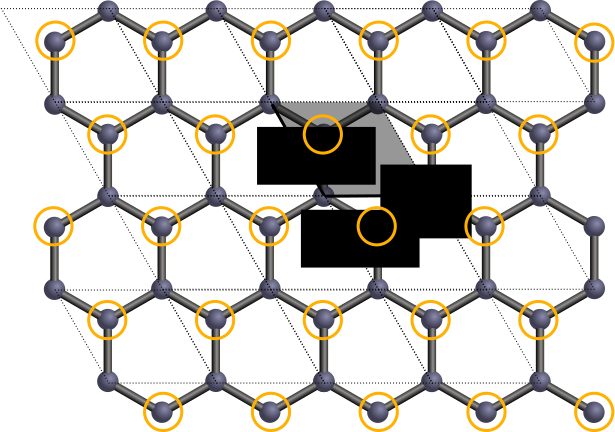
\includegraphics[width=0.8\textwidth]{graphite-lattice}
	\caption{Graphite structure}
	\label{fig:graphite-lattice}
\end{figure}

In three dimension this lattice general arguments extends but the vector that represents all positions in the lattice get an extra term as usual
\begin{equation}
	\mathbf{r}_{uvw} = u\mathbf{a} + v\mathbf{b} + w\mathbf{c}
	\label{eq:crystal-lattice-3d}
\end{equation}
and instead of getting an area as covered in grey by $\mathbf{a}$ and $\mathbf{b}$ in figure~\ref{fig:graphite-lattice}, we get a volume, a volume we call the \textbf{unit cell}.

\subsubsection{lattice symmetries}
The lattice symmetries are usually important when looking at the property of a certain solid. In turns out the available possibilities are quite limited too. We lattices such as the \textbf{rectangular lattice}, \textbf{rhombic lattice} and the \textbf{centred rectangular lattice}. Look in the book for further explanation.

\subsubsection{The basis}\label{sec:basis}
The basis is what we use to define a position of a particular atom within a lattice. For our example in figure~\ref{fig:graphite-lattice} we have vector 
\begin{equation}
	\mathbf{r}_b = \frac{2}{3}\mathbf{a} + \frac{1}{3} \mathbf{b}
	\label{eq:basis}
\end{equation}
that defines the position of the yellow circled atom from a lattice point. But the basis also describes the type of atom, thus we end up with the basis 
\begin{equation}
	C(0,0),C(\frac{2}{3}, \frac{1}{3})
\end{equation}
where the first $C$ defines the atom at the lattice point, and the second the other atom which was on on the lattice ($C$ specifies that it is a carbon atom).
Likewise for a three dimensional structure we just add one simple term for the position. 

Taking the symmetry of the basis as well as the crystal lattice, we can sort a crystal into on of the 32 possible \textbf{point symmetry groups} or \textbf{crystal classes} and one of the 230 possible \textbf{space symmetry groups}.

\subsubsection{Crystal planes and directions}
Imagine we have a three dimensional rectangular lattice(incidently called a cubical lattice) that we depict in two dimensions as we have done in figure~\ref{fig:lattice-planes}. We can then define a multitude of planes that goes through multiple lattice points. In two dimension in looks simply like lines, but if we stretch that out in three dimensions we can easily see the planes, which is more clearly depicted in figure~\ref{fig:lattice-planes-3d}.
\begin{figure}[H]
	\centering
	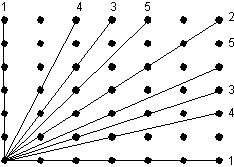
\includegraphics[width=0.8\textwidth]{lattice-planes}
	\caption{Some lattice planes in the cubic lattice, depicted in two dimensions}
	\label{fig:lattice-planes}
\end{figure}
\begin{figure}[H]
	\centering
	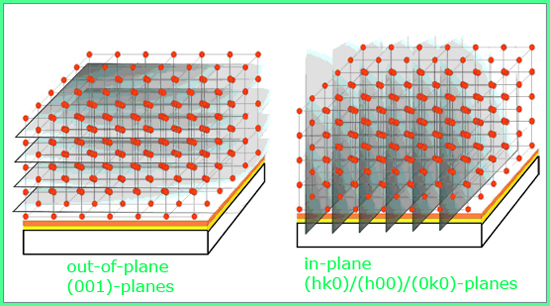
\includegraphics[width=0.8\textwidth]{lattice-planes-3d}
	\caption{Some lattice planes in the cubical lattice, now in 3D!}
	\label{fig:lattice-planes-3d}
\end{figure}

\newpage
These lattice planes plays an important role in the diffraction of incoming waves (usually light or more generally an electromagnetic wave). Thus it's important to identify different sets. This in done through \textbf{Miller indicies}. These indices are defined through where a plane intersects the crystal axes closest to it's origin, but not through the origin. By looking at figure~\ref{fig:lattice-planes-vis} we can see four different examples. If we let $\mathbf{a} = x$, $\mathbf{b}=y$ and $\mathbf{c} =z$ we can see how in (d) how we have a plane that intersects the crystal axes at $(\frac{\mathbf{a}}{1},\frac{\mathbf{b}}{1}, \frac{\mathbf{c}}{2})$. The Miller Indices is then the reciprocal of these factors we multiply the crystal axes with in order to find the intersect point, it's written as $(1 1 2)$. if a plane is parallel to a particular axis it's taken at a zero. 

\begin{figure}[H]
	\centering
	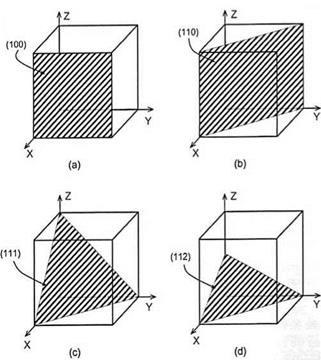
\includegraphics[width=0.8\textwidth]{lattice-planes-vis}
	\caption{Some lattice planes in the rectangular lattice, visually in 3d!}
	\label{fig:lattice-planes-vis}
\end{figure}

\newpage
We should also note that from an atomic view a certain amount of planes could due to symmetry in the crystal lattice be equivalent to eachother. This is depicted in figure~\ref{fig:lattice-planes-symmetry}. All these three planes are said to belong to the \textbf{form} $\{100\}$.
\begin{figure}[H]
	\centering
	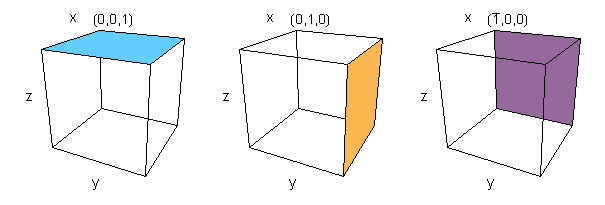
\includegraphics[width=0.8\textwidth]{lattice-planes-symmetry}
	\caption{These lattice planes is equivalent from an atomic point of view, thus all these three are written as belonging to the form $\{100\}$}
	\label{fig:lattice-planes-symmetry}
\end{figure}

One often want to specify the directions of a vector $\mathbf{r}$ in a crystal. A vector can be written as 
\begin{equation}
	\mathbf{r} = u\mathbf{a} + v \mathbf{b} + w \mathbf{c}
\end{equation}
We then refer to it as the $[uvw]$ direction. Due to symmetry in cubic crystals the $[uvw]$ direction is actually the normal to the $(uvw)$ plane. It should however be noted that this an exception and only hold for lattices with the particular symmetries of the cubic lattice.

\newpage
\subsection{Typical crystal structures}
Imagine that the atoms act like spheres, so if we wanna tightly pack them it's like packing cannon balls\footnote{This is actually very close to the truth since the atoms interact with each other with a force that is radial.}. This is depicted in figure~\ref{fig:packed-spheres}. The layer depicted can be stacked upon with another layer with spheres in the A,B or C positions. Now packing the other layer on the A position is neither stable nor efficient, and something that generally don't happen in nature. But depending on how the stacking structure looks like in an atom the solid gets a different structure which can be described by different lattices. 
\begin{figure}[H]
	\centering
	\includegraphics[width=0.8\textwidth]{packed-spheres}
	\caption{packed spheres! in 2d!}
	\label{fig:packed-spheres}
\end{figure}
\subsubsection{Cubic and hexagonal close-packed structures}
The ABCABC\ldots stacking yields the \textbf{face-centred cubic} structure, its conventional non-primitive unit cell is depicted in figure~\ref{fig:fcc}.
\begin{figure}[H]
	\centering
	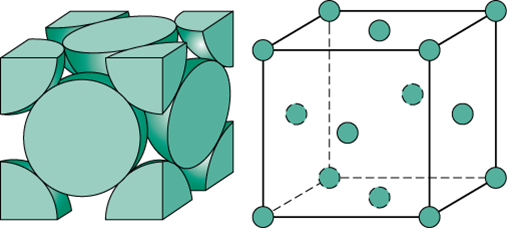
\includegraphics[width=0.8\textwidth]{fcc}
	\caption{The face centred cubic}
	\label{fig:fcc}
\end{figure}
\subsubsection{The body-centred cubic structure}
The body centred cubic structure is not quite close packed, so has no real equivalent to the packing sequence as the fcc does. This is due to certain positions are missing in this structure. In reality we can defend this lack of atoms due to the repelling forces among the atoms. The structures conventional non-primitive cell is depicted in figure~\ref{fig:bcc}.
\begin{figure}[H]
	\centering
	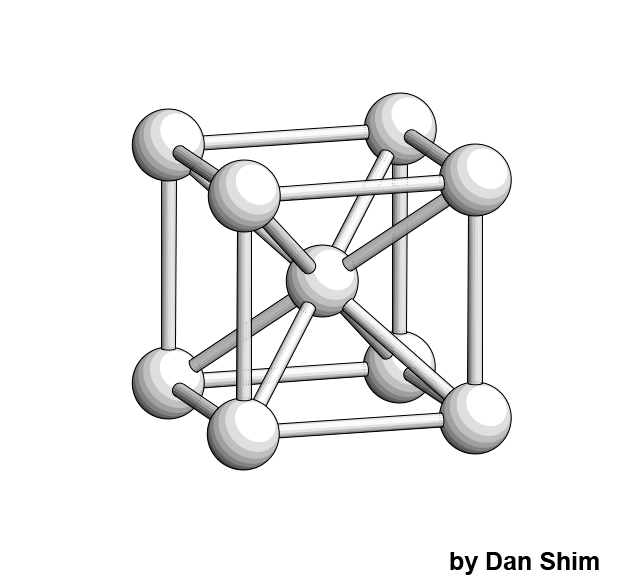
\includegraphics[width=0.8\textwidth]{bcc}
	\caption{The body centred cubics non-primitive conventional cell}
	\label{fig:bcc}
\end{figure}

\newpage
\subsubsection{Structures of ionic solids}
Ionic soldis are simply a crystal containing more then one element(or a specific type of an atom as we will more specifically look at). In figure~\ref{fig:nacl} we can see atomic structure of the NaCl molecule.  EElectrons in the negatively charged anion(Cl) are generally less tightly bund than those in the positively charge anion(Na). By convention we write the lously bounded anion as the bigger atom in our structure. 

It's interesting to note that we have $(111)$ planes in this lattice as showed here which will create planes of only Na or Cl atoms. That can be showed through it's diffraction properties. 
\begin{figure}[H]
	\centering
	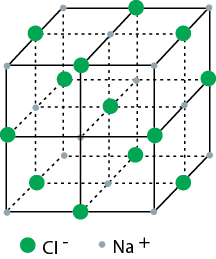
\includegraphics[width=0.8\textwidth]{nacl}
	\caption{The ionic structure of the NaCl solid}
	\label{fig:nacl}
\end{figure}
\newpage
\subsubsection{The diamond and zincblende structures}
A more advanced structure which basically can be constructed through a cubic lattice and a more complex basis. This structure is showed in figure~\ref{fig:zincblende-structure}. It's interesting that the structure is identitical for zincblende and diamonds, the only difference is that diamonds are only carbon, while zincblende is made from zinc and  sulfur.
\begin{figure}[H]
	\centering
	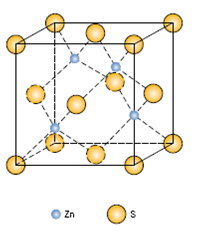
\includegraphics[width=0.8\textwidth]{zincblende-structure}
	\caption{The structure for zincblende. Note that it's the same for diamonds except for diamonds you only have carbon}
	\label{fig:zincblende-structure}
\end{figure}

\newpage
\subsubsection{The Wigner-Seitz cell}
By taking the planes that goes perpendicularly  through all the bisects of the lines to an atoms neighbours, one end up with its Wigner-Seitz cell. This represents the "sphere of influence". For the fcc such a cell has twelve neighbours and twelve faces, thus all the sites in fcc has a \textbf{coordination number} of twelve.

Always a primitive cell.
\begin{figure}[H]
	\centering
	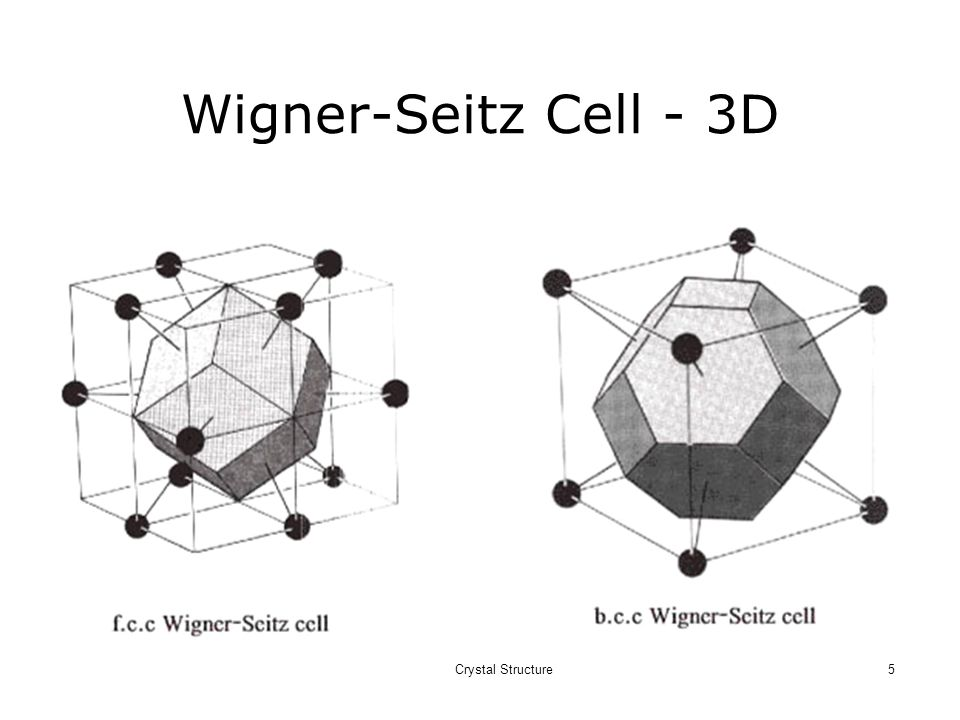
\includegraphics[width=0.8\textwidth]{wigner-seitz}
	\caption{The Wigner-Seitz cell for the fcc and bcc structure}
	\label{fig:wigner-seitz}
\end{figure}

\newpage
\subsection{X-ray crystallography}
\subsubsection{The Bragg  law}
Bragg law is a simplified way of looking at the reflection from crystal structures. Instead of using the general laws of diffraction as von Laue did, we will just see lattice planes as "reflective planes". One can then use Braggs law to help identify crystal structures
\begin{equation}
	2d\sin{\theta} = n\lambda
\end{equation}
We can have reflections of higher orders ($n>1$). If we for instance get a reflection of the third order from the plane $(111)$ we call it through convention the reflection of plane $(333)$. In general terms a nth order reflection of a plane $(hkl)$ is written as a reflection from plane (nh nk nl).

\begin{figure}[H]
	\centering
	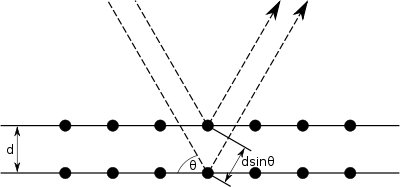
\includegraphics[width=0.8\textwidth]{bragg}
	\caption{The reflection due to lattice planes}
	\label{fig:bragg-law}
\end{figure}

\subsubsection{Experimental arrangements for x-ray dirffraction}
\newpage
\paragraph{A Laue photograph} is depicted in figure~\ref{fig:laue-photograph}. It is usually a good at showing symmetries, thus a good tool for figuring out the orientation of a crystal.
\begin{figure}[!h]
	\centering
	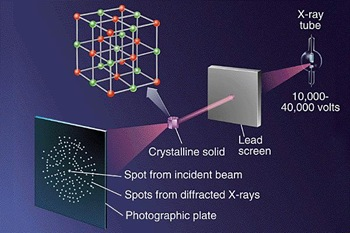
\includegraphics[width=0.8\textwidth]{laue-photograph}
	\caption{The experimental setup for the Laue photograph}
	\label{fig:laue-photograph}
\end{figure}

\newpage
\paragraph{A Rotating crystal and powder photograph} is depicted in figure~\ref{fig:rotating-crystal}. It's a tool better suited for analysing the actual structure of a crystal.
\begin{figure}[!h]
	\centering
	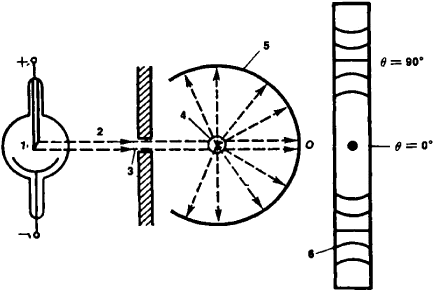
\includegraphics[width=0.8\textwidth]{rotating-crystal}
	\caption{The basic setup for a rotating crystal photograph or powder photograph. The difference is wether on not the speciment in the middle is a rotating crystal or a powder of crystalline crystals.}
	\label{fig:rotating-crystal}
\end{figure}

\newpage
\subsection{Interatomic forces}
\subsubsection{Van der Waals bonding}
Van der Waals occurs with even stable atoms, those who has all the outer electrons in their shell. This is due to flutuation that creates an electric dipole moment. This force experienced is described by the Lennard-Jones potential depicted in figure~\ref{fig:lennard-jones}. Worth noting that the repulsive force is a consequence of the Pauli principle, that states that no two electrons can occupy the same state, and instead the electrons get excited to higher state if another one would come close. This creates a large repulsive force which one clearly see in the Lennard-Jones potential.
\begin{figure}[!h]
	\centering
	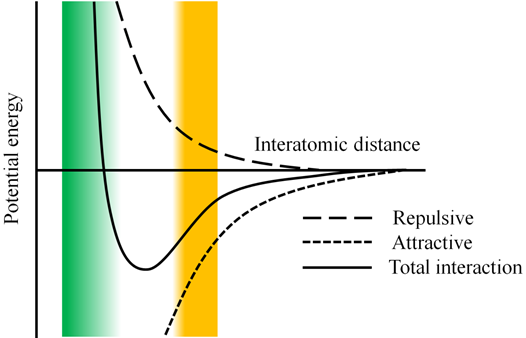
\includegraphics[width=0.8\textwidth]{lennard-jones}
	\caption{The Lennard-Jones potential is the main force in Van der Waals bonding. The color green represent a distance in which repulsion occurs, while the color of orange represents a distance of attraction. Kinda like how it is with us humans too lol.}
	\label{fig:lennard-jones}
\end{figure}

\newpage
\subsubsection{Ionic bonding}
Basically ionic bonding is the process of atoms sharing one electron in order to create two charged atoms with completed outer shells. The truth goes of course down too Schrödinger's, but in this is as far as we go to it now.
\begin{figure}[!h]
	\centering
	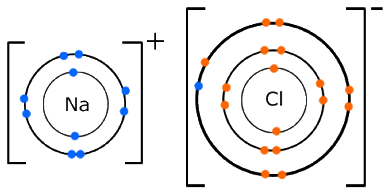
\includegraphics[width=0.8\textwidth]{ionic-bond}
	\caption{The ionic bond between Na and Cl. In this example Na gives away its stray atom in its outer shell in order to complete the outer shell of Cl. The reality is more complex, but deeply related to electron states in the shells.}
	\label{fig:ionic-bond}
\end{figure}

\newpage
\subsubsection{Covalent bonding}
The covalent bonding is similar to the ionic bonding in the sharing of electrons. The covalent bond has some more complexity related to it. It's usually directed too, so can, among other things, be a factor of why there exists solids which has more complex structures. Basically atoms can share electrons between multiple atoms in order for all the outer shells to saturated. This is depicted in figure~\ref{fig:covalent} for the famous $H_2O$ molecule.

\begin{figure}[!h]
	\centering
	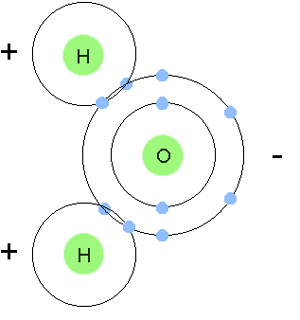
\includegraphics[width=0.8\textwidth]{covalent}
	\caption{The covalent bond is similar to the ionic bond, but shares multiple electrons, could be over multiple atoms and those usually have some kind of direction related to it.}
	\label{fig:covalent}
\end{figure}

\subsubsection{Hydrogen bonding}
Looking at the earlier picture of the $H_2O$ molecule in figure~\ref{fig:covalent}, we can see that the molecule itself has a negative and positive charge. This causes important bindings in ice and many organic solids.

\newpage
\subsubsection{Metallic bonding}
In the metallic bond we have a kind of covalent bond which does not saturate the outer shell of the atoms. This results in "wandering atoms" as depicted in figure~\ref{fig:metallic-bonding}. This in turns facilitate the ability to conduct electricity. 
\begin{figure}[!h]
	\centering
	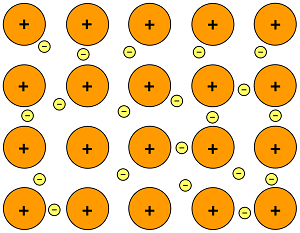
\includegraphics[width=0.8\textwidth]{metallic-bonding}
	\caption{In the metallic bond the atoms share their electrons more freely}
	\label{fig:metallic-bonding}
\end{figure}

\newpage
\subsubsection{Mixed bonding}
Basically just highlighting that we can more then one bond in a solid. As an example we have graphite as depicted in figure~\ref{fig:graphite-bond}. There we have both a covalent bond in the layer, as well a Van der Waals bond between layers. This causes graphite to have the interesting effect of only conducting electricity in the direction parallel to the layers, not perpendicular to it (and thus the Van der Waals bond does not conduct electricity especially well).
\begin{figure}[!h]
	\centering
	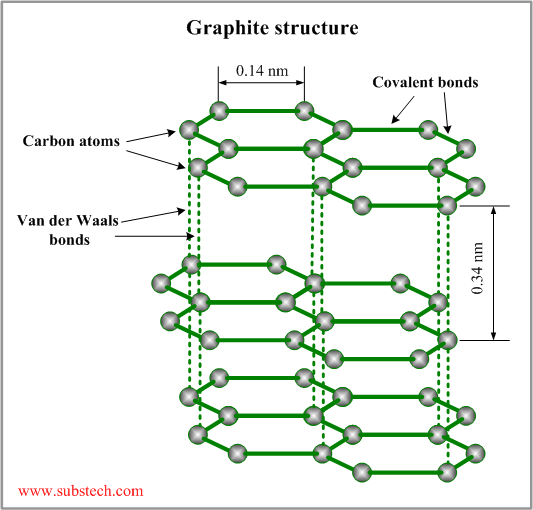
\includegraphics[width=0.8\textwidth]{graphite-bond}
	\caption{Depicting the mixed bond inside graphite. Each layer has strong covalent bond, while between layers only Van der Waals forces keeps it together.}
	\label{fig:graphite-bond}
\end{figure}
\newpage 
\subsection{New Words}

\begin{itemize}
	\item \textbf{crystal lattice}
	\item \textbf{translational invariance}
	\item \textbf{unit cell}
	\item \textbf{rectangular lattice}
	\item \textbf{rhombic lattice}
	\item \textbf{centred rectangular lattice}
	\item \textbf{point symmetry groups}
	\item \textbf{crystal classes} 
	\item \textbf{space symmetry groups}
	\item \textbf{Miller indicies}
	\item \textbf{face-centred cubic}
	\item \textbf{coordination number}
\end{itemize}

\newpage
\section{Waves in crystals}

\subsection{Elastic scattering of waves by a crystal}
\subsubsection{Amplitude of the scattered wave}
Using braggs law we were able to find where we should have reflections. But we know nothing of the amplitude. This we will find out by examining every atom as a point source for radial radiation. This radial radiation gets created when excited, or radiation has hit it. The setup for this thought process is depicted in figure~\ref{fig:crystal-plane-wave}. 

Lets assume the incident radiation is a plane wave on the form $A_0 \exp{[i(\mathbf(k) \cdot \mathbf{r} - \omega t)]}$. The resulting amplitude of the radiation at the detector is then
\begin{equation}
	A_r = A_0 e^{i(\mathbf{k} \cdot \mathbf{r} - \omega t)} \times f \times \frac{e^{ik(|\mathbf{R} - \mathbf{r}|)}}{|\mathbf{R}-\mathbf{r}|}.
\end{equation}

\begin{figure}[!h]
	\centering
	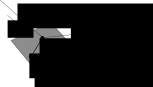
\includegraphics[width=0.8\textwidth]{crystal-plane-wave}
	\caption{An incoming plane wave towards a crystal and description of what part radial excitation wave will hit the detector}
	\label{fig:crystal-plane-wave}
\end{figure}

We can see three terms in the right hand side of this equation. We will number them as they appear in the equation. The first part is just the incoming wave. The second part is the \textbf{atomic form factor} or \textbf{atomic scattering factor}, which defines how much radiation a certain atom will scatter. The third term is the apmlitude decrese and phase change due to the position of an atom. Assuming that the distance of the detector from the crystal is insanely much larger then the crystal atom distances we can simplify the third term to be
\begin{equation}
	\frac{e^{ik(|\mathbf{R} - \mathbf{r}|)}}{R}.
\end{equation}
We go on to define the \textbf{scattering vector} $\mathbf{K}$ as 
\begin{equation}
	\mathbf{K} = \mathbf{k}'-\mathbf{k}
\end{equation}
We can also apparently sag that $k \cdot |\mathbf{R}-\mathbf{r}| \approx \mathbf{k}'\cdot (\mathbf{R}-\mathbf{r})$. So we end up with a term for the amplitude as 
\begin{equation}
	A_r \approx A_0 \frac{e^{i(k\mathbf{R}-\omega t)}}{R} f e^{-i\mathbf{K} \cdot \mathbf{r}}
\end{equation}
The first term in this equation is the same for all atoms in a structure, so it can be factored out as a constant. We are left with knowing that the amplitude is proportional to
\begin{equation}
	A = \sum_n f_n e^{i\mathbf{K} \cdot \mathbf{r}_n}
\end{equation}
where the sum is over all atoms in the crystal.

Recalling that the position of an atom can be made up of lattice point position and its basis inside that we can split $\mathbf{r}$ into its lattice association $\mathbf{r}_l$ and position relative to the lattice point(using the basis) $\mathbf{r}_p$. This idea is depicted in figure~\ref{fig:basis-sep}. The equation then becomes
\begin{equation}
	A = \sum_l  e^{i\mathbf{K} \cdot \mathbf{r}_l} \times \sum_p f_p e^{i\mathbf{K} \cdot \mathbf{r}_p}
	\label{eq:ampl}
\end{equation}
The first part of this right hand expression is what determines the direction for which diffraction occurs and is due to the crystal lattice. The second part is due to the basis, and is the same for all lattice points, which is a sum over relatively few atoms. This second part is called the \textbf{structure factor}.

\begin{figure}[!h]
	\centering
	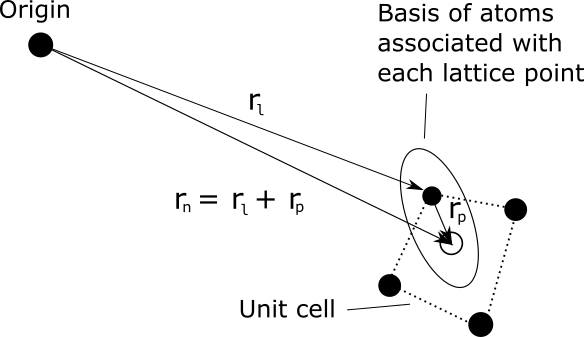
\includegraphics[width=0.8\textwidth]{basis-sep}
	\caption{}
	\label{fig:basis-sep}
\end{figure}

\newpage
\subsubsection{Laue conditions for diffraction and the reciprocal lattice}
Using equation~\ref{eq:crystal-lattice-3d} for the crystal lattice, and the first term in equation~\ref{eq:ampl} we get
\begin{equation}
	\sum_l e^{i\mathbf{K} \cdot \mathbf{r}_l} =\sum_u e^{i\mathbf{K} \cdot \mathbf{a}u} + \sum_v e^{i\mathbf{K} \cdot \mathbf{b}_v} + \sum_w e^{i\mathbf{K} \cdot \mathbf{c}w}.
\end{equation}
Since we only get a large scattering amplitude when the contribution from all the lattice point are in phase, we get the requirement that
\begin{align}
	\mathbf{K} \cdot \mathbf{a} &= 2\pi h \\
	\mathbf{K} \cdot \mathbf{b} &= 2\pi k \\
	\mathbf{K} \cdot \mathbf{c} &= 2\pi l 
\end{align}
where $h,k,l$ is integers. This is what we call the \textbf{Laue conditions} for diffraction. When these requirements are satisfied we get unity from the lattice term in amplitude for every lattice point and we end up with the number of primitive unit cells as the lattice term.

The directions of the diffracted beams are thus given by the set of vectors $\mathbf{k}$ that satisfies the Laue conditions. It turns out that this set of vectors are actually the reciprocal of the lattice vectors! I.e.
\begin{equation}
	\mathbf{K} = h\mathbf{a^*} + k\mathbf{b^*} + l \mathbf{c^*}
\end{equation}
where 
\begin{align}
	\mathbf{a^*} &= \frac{2\pi(\mathbf{b}\times\mathbf{c})}{\mathbf{a}\cdot(\mathbf{b}\times\mathbf{c})} \nonumber\\
	\mathbf{b^*} &= \frac{2\pi(\mathbf{c}\times\mathbf{a})}{\mathbf{a}\cdot(\mathbf{b}\times\mathbf{c})} \nonumber\\
	\mathbf{c^*} &= \frac{2\pi(\mathbf{a}\times\mathbf{b})}{\mathbf{a}\cdot(\mathbf{b}\times\mathbf{c})} 
	\label{eq:reciprocal-lattice}
\end{align}
The book proves in page 321 that braggs and this requirements both holds up.

Since the scattering vector of each diffracted beam corresponds to a point in reciprocal lattice, we can use the integers $h,k,l$ to label the beams. These labels are identical to the miller indices of the lattice plane that is associated with the diffracted beam, this is also proved in the book at page 321.   

To surmise: for an incident radiation of wavevector $\mathbf{k}$, the direction of the diffracted beams are given by wavevectors $\mathbf{k'} = \mathbf{k} + \mathbf{K}$, where the scattering vector $\mathbf{K}$ is any one of the points of the reciprocal lattice for the crystal. You determine the $\mathbf{K}$ vector through equations~\ref{eq:reciprocal-lattice}.

\subsubsection{Examples of reciprocal lattices}
In describing these reciprocal we will use the three mutually perpendicular real value unit vectors $mathbf{i}$, $mathbf{j}$, $mathbf{k}$.
\paragraph{The simple cubic real space lattice} is going to be investigated first!
In terms of Cartesian axes we have 
\begin{align}
	\mathbf{a} &= a\mathbf{i} \nonumber\\
	\mathbf{b} &= a\mathbf{j} \nonumber\\
	\mathbf{c} &= a\mathbf{k} 
\end{align}
using equation~\ref{eq:reciprocal-lattice} we get the reciprocal

\begin{align}
	\mathbf{a} &= \frac{2\pi}{a}\mathbf{i} \nonumber\\
	\mathbf{b} &= \frac{2\pi}{a}\mathbf{j} \nonumber\\
	\mathbf{c} &= \frac{2\pi}{a}\mathbf{k}  
\end{align}
Basically just the same with shorter sides!

\newpage
\paragraph{The face-centred cubic real space lattice} is intriguingly connected with the bcc. We start with define the fcc as
\begin{align}
	\mathbf{a} &= \frac{a}{2} (\mathbf{j} + \mathbf{k}) \nonumber\\
	\mathbf{b} &= \frac{a}{2} (\mathbf{k} + \mathbf{i}) \nonumber\\
	\mathbf{c} &= \frac{a}{2} (\mathbf{i} + \mathbf{j}) 
\end{align}
which gives us the reciprocal
\begin{align}
	\mathbf{a} &= \frac{2\pi}{a} (\mathbf{j} + \mathbf{k} - \mathbf{i}) \nonumber\\
	\mathbf{b} &= \frac{2\pi}{a} (\mathbf{k} + \mathbf{i} - \mathbf{j}) \nonumber\\
	\mathbf{c} &= \frac{2\pi}{a} (\mathbf{i} + \mathbf{j} - \mathbf{k}) \nonumber\\
\end{align}
Which yields the bcc! Not completely visible perhaps, maybe easier to see through the reciprocal equations directly perhaps. But basically the vectors get translated around to the bbc, and scaled of course, this is depicted in figure~\ref{fig:fcc-bcc}.
\begin{figure}[!h]
	\centering
	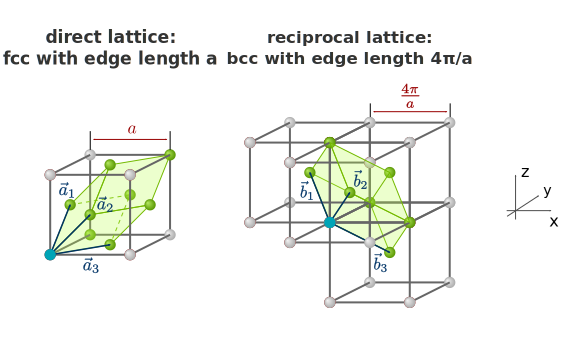
\includegraphics[width=0.8\textwidth]{reciprocal-lattice-fcc-bcc}
	\caption{Here we can see how the reciprocal of the fcc lattice is just rotated and scaled into a bcc lattice}
	\label{fig:fcc-bcc}
\end{figure}

\newpage
\subsubsection{The structure factor}
Now it's time we look at the second part of equation~\ref{eq:ampl}. This part 
\begin{equation}
	S = \sum_p f_p e^{-i\mathbf{K} \cdot \mathbf{r}_p}
	\label{eq:structure-factor}
\end{equation}
is known as the structure factor and only concerns the basis in the structure. 

\paragraph{The simplest form} of structure factor occurs when we only have one atom at each lattice point. This then reduces to be 
\begin{equation}
	S = f
\end{equation}
where f is only dependent on the incident angle and what kind of atoms that occurs on the lattice.

\newpage
\paragraph{Using the hexagonal close packed structure}, as depicted in figure~\ref{fig:hcp}, we get another basis 
\begin{align}
	\mathbf{r}_1 &= \mathbf{0} \\
	\mathbf{r}_2 &= \mathbf{a}/3+\mathbf{b}(2/3) + \mathbf{c}/2
\end{align}
So if we put this into the structure factor equation~\ref{eq:structure-factor} and use the reciprocal equation~\ref{eq:reciprocal-lattice}, we get
\begin{equation}
	S = f\{1+\exp{[-i\pi((h+k+l)+(k-h)/3)]}\}
\end{equation}
Since the amplitude is proportional to $S$, we can use this equation to do some analysis of where the amplitude might completely go to zero. But also to some extend see which planes will have a large contribution to reflections. This of course have to weighted against the lattice term as well.

We also have to note we haven't looked into the atomic factor at all. It could differ for the same atoms as well due to different environment and such. This have an effect on structures like the diamond.
\begin{figure}[!h]
	\centering
	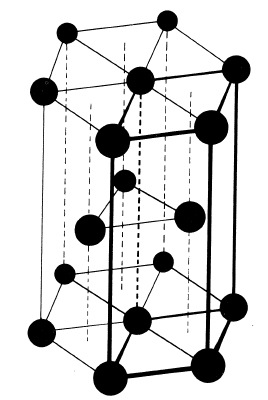
\includegraphics[width=0.4\textwidth]{hcp}
	\caption{The hexagonal close packed structure.}
	\label{fig:hcp}
\end{figure}

\newpage
\section{Diamagnetic and paramagnetism}
\subsection{Introduction}
The increase in a magnetic field applied to any material\footnote{referred to as $\mathbf{H}$} causes an induced electromotive force, which in turn accelerates electrons in the material. Then according to Lenz's law the resulting electric current is such that it reduces the magnetic field applied inside the material, one also say that the magnetic field is ``screened'' from the material.

What's more interesting is that this current actually still exist even if the magnetic field is held at a constant value\footnote{We will explain this phenomenon later.}. If this does indeed happen in a material, then the material is \emph{diamagetic}. Note that the current creates a magnetic field, Denoted as $\mathbf{M}$, which works against the applied magnetic field, $\mathbf{H}$.

If a material posses atoms with a permanent magnetic dipole moment\footnote{Think bar magnets.}, then the diamagnetic effects are usually very small in comparison to the \emph{paramagnetic} effects. The paramagnetic effect creates a magnetization, $\mathbf{M}$, which works with the applied magnetic field, $\mathbf{H}$. 

We can relate the magnetization of the material, $\mathbf{M}$, with the applied magnetic field, $\mathbf{H}$ through the magnetic susceptibility, $\chi$, of the material as 
\begin{equation}
	\mathbf{M} = \chi \mathbf{H}.
\end{equation}
From this we can deduce the sign of the magnetic susceptibility will be positive for paramagnetic materials and negative for diamagnetic materials. 

\subsection{Paramagnetism}
\subsubsection{The origin of permanent dipole moments}
From ampere's law we can deduce an equation for the magnetic dipole moment, $\pmb{\mu}$, to be
\begin{equation}
	\pmb{\mu} = i \pmb{a}.
\end{equation}
Where $\pmb{a}$ is the area vector of the loop, directed so that the current is clockwise when looking along $\pmb{a}$. and $i$ is the electric current.

To start with we can look at the dipole moment of a electron going around it's nucleus with a period of $\tau$, and a radius $r$. The current is then 
\begin{equation}
	i = (-e)/\tau = -e v/2\pi r.
\end{equation}
Where the negative sign comes from the fact that the electron moves in the opposite direction of the current\footnote{Thank you convention for making everything confusing!}. Rewriting the dipole moment with this current we get
\begin{equation}
	\pmb{\mu} = - \frac{ev}{2\pi r} \pmb{a}.
\end{equation}
Now we can use the angular moment of the electron which is $\hslash \pmb{I}$. The $\hslash$ is just convention, as we know constants can be multiplied in and divided away as long as it's done in a balanced matter. If we see that $|\pmb{a}| = \pi r^2$, $|\hslash| = mvr$ and that $\pmb{a}$ and $\pmb{I}$ is directed in the same direction, we can rewrite the dipole moment as
\begin{equation}
	\pmb{\mu} = - \frac{e\hslash}{2m} \pmb{I}.
	\label{eq:orbital_momentum}
\end{equation}
We can then define the constant part as the Bohr magneton, $\mu_B$, i.e.
\begin{equation}
	\mu_B = \frac{e\hslash}{2m} = 9.27 \times 10^{-24} J T^{-1}.
\end{equation}

Now we've used the classical model of an electron spinning around its nucleus to figure out the dipole moment contribution due to the orbital angular momentum of the electron through equation~\ref{eq:orbital_momentum}. But due to hand waviness, we're gonna go the quantum mechanical route with this equation. Thus we have an equation 
\begin{equation}
	\pmb{\mu} = -\mu_B \pmb{I}
\end{equation}
for the orbital angular momentum, but also a magnetic dipole moment is given for the spin in the quantum mechanical treatment that is as follows
\begin{equation}
	\pmb{\mu_{spin}} = - g_0 \mu_B \pmb{S}.
\end{equation}
And we estimate $g_0=2$\footnote{Sorry, too intricate to explain} and we get a total magnetic dipole moment to be
\begin{equation}
	\pmb{\mu} = - \mu_B (\pmb{L}+2\pmb{S}).
	\label{eq:total_angular_momentum}
\end{equation}
Where $\pmb{L}$ is the total sum of atoms electron orbital momentums and $\pmb{S}$ is the sum of the atoms electrons spin angular momenta. For every closed shell this sum adds up to be zero. Thus permanent dipole moments only occur in atoms or ions with an incomplete shell. 

To look at how an incomplete shell is built for incomplete shells in isolated ions, and thus being able to calculate the momenta of them, we use the Russell-Sounders coupling scheme, or L-S coupling. It states that the stationary states of the shell are eigenstates of $\pmb{L^2}, \pmb{S^2}$ and $\pmb{J^2}$, with eigenvalues $L(L+1), S(S+1)$ and $J(J+1)$. To find the values of L,S and J we use the Hund's rules
\begin{enumerate}
	\item S takes the maximum value allowed by the exclusion principle, thus as many as possible of the electrons have parallel spins
	\item L takes the maximum value consistent with this value of S - the electrons have their orbital angular momenta as well aligned as possible
	\item $J = |L-S|$ for shells less then half full and $J = L+S$ for shells more then half full.
\end{enumerate}

Here it's interesting to note that rule 1 and 2 of Hund's rules are closely associated with the Coulomb forces between electrons, due to them being much larger then the magnetic force\footnote{Not argued for here, but take my word for it!}. And the value of j, is associated with the spin-orbit interaction, that is with the magnetic field generated by the motion of the electrons within the atom, this is of order 10T\footnote{Also just a given fact}. So the 3rd rule can be effected by a field applied of this order.

In figure~\ref{fig:hunds} we get a picture of two ions having applied the Hund's rule on to determine the values of L,S and J. 

\begin{figure}[!h]
	\centering
	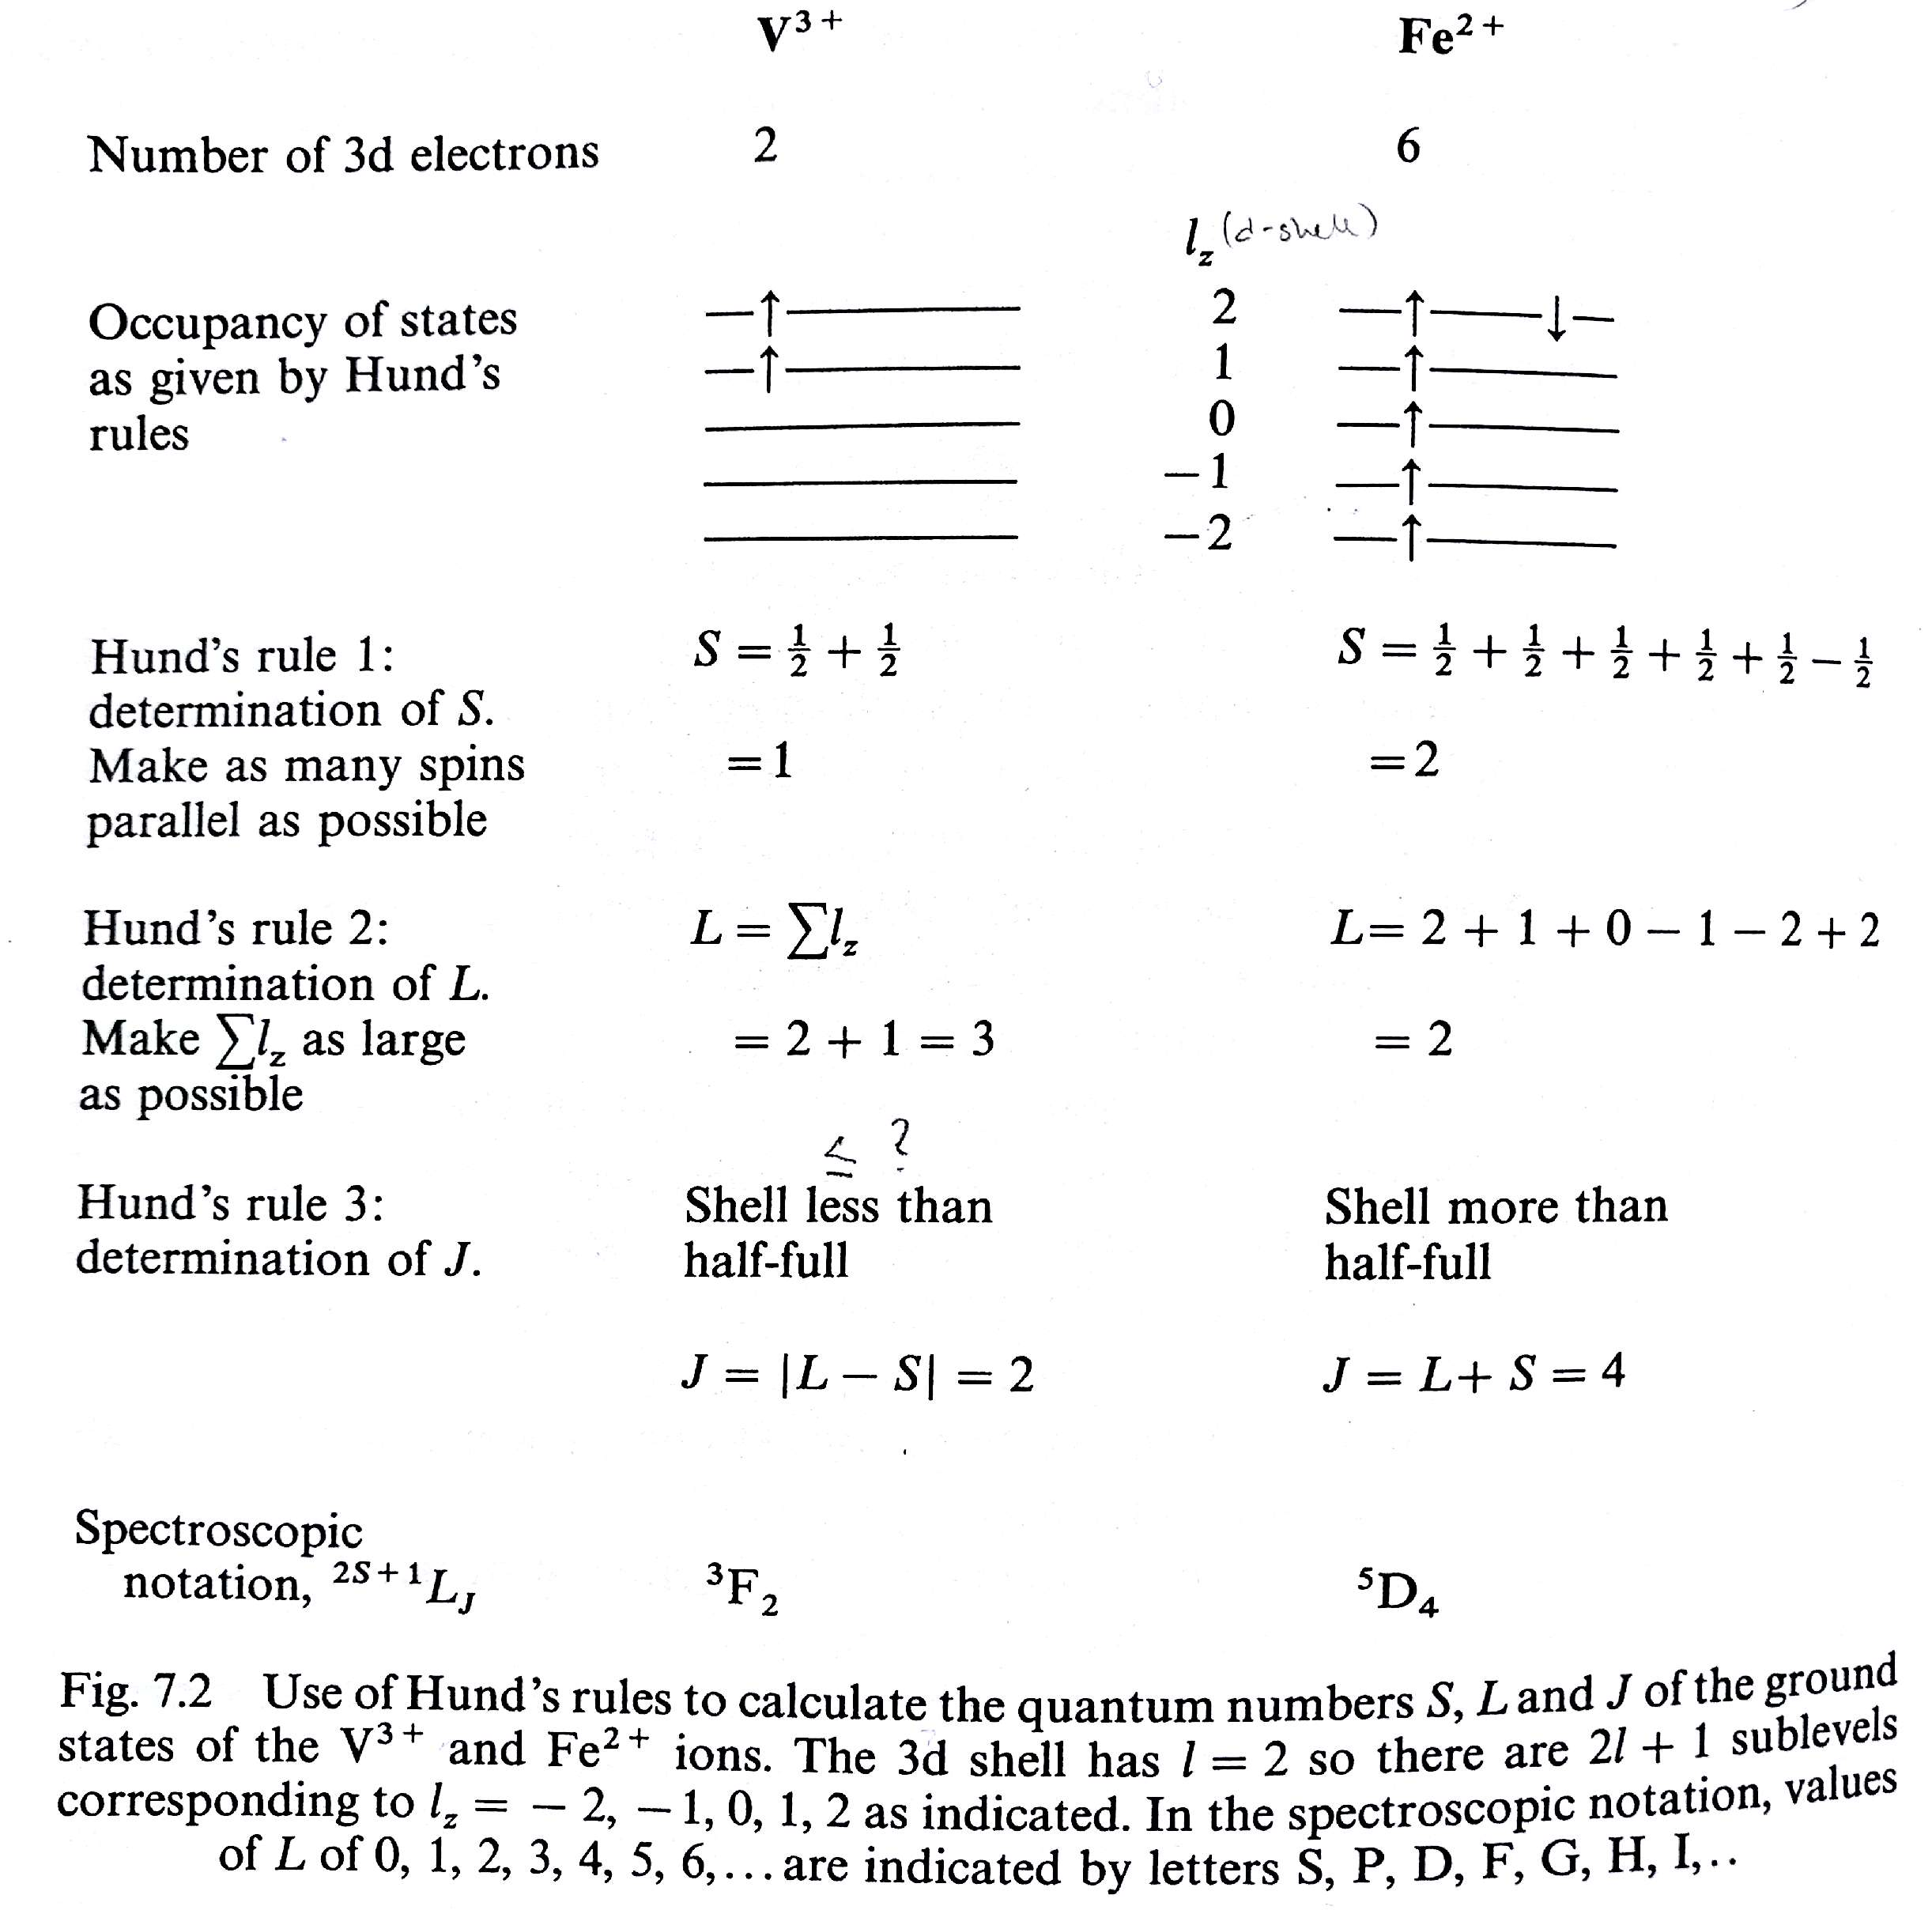
\includegraphics[width=\textwidth]{hunds}
	\caption{Copied from Solid State Physics by J.R. Hook and H.E. Hall}
	\label{fig:hunds}
\end{figure}

\subsubsection{The interaction of permanent dipole moment with an applied magnetic field}
Alignment of an atomic dipole by a field $\pmb{B}$ (which is taken to be along the z-axis) occurs because of an energy term in the electrons, $H_P$,
\begin{equation}
	H_P = - \pmb{\mu} \cdot \pmb{B} = -\mu_z B.
	\label{eq:alignment_energy}
\end{equation}
Where $\pmb{\mu}$ is given by equation~\ref{eq:total_angular_momentum}. It should however be noted that you should not think of it as an atomic bar magnet, because things does not quite act on the atomic level as things does in the macroscopic world. 

\newpage
If we assume that the energy $H_p$ is small, we can use first-order perturbation theory to calculate the effect of the alignment energy. We then assume a ground state for the ion, or atom, we look at (nothing excited to a new level) and use quantum hand waviness to get the expectation energy
\begin{equation}
	\langle H_p \rangle = g\mu_B J_z B
	\label{eq:expected_alignment_energy}
\end{equation}
where $j_z = -j,\ldots ,1,0,1,\ldots j$ and g is the \emph{Landé g-factor} 
\begin{equation}
	g = \frac{3}{2} - \frac{L(L+1) - S(S+1)}{2J(J+1)}
\end{equation}

Comparing equation~\ref{eq:alignment_energy} and equation~\ref{eq:expected_alignment_energy}, we can see that we seem to have an effective magnetic moment 
\begin{equation}
	\pmb{\mu}_{eff} = g\mu_B\pmb{J}
\end{equation}
\subsubsection{Calculation of the magnetization of paramagnetic ions}
\subsubsection{Conduction electron paramagnetism}

\subsection{Diamagnetic}
\subsubsection{Momentum in a magnetic field}
\subsubsection{Screening by induced currents}
\subsubsection{Calculation of the diamagnetic susceptibility}

\subsection{New words}
\begin{itemize}
	\item \textbf{Diamagnetism}
	\item \textbf{Paramagnetism}
	\item \textbf{Magnetic susceptibility - $\chi$}
	\item \textbf{Magnetization - $\mathbf{M}$}
	\item \textbf{Macroscopic magnetic field within a material - $\mathbf{H}$}
\end{itemize}


\newpage
\begin{thebibliography}{9}
\end{thebibliography}
\clearpage
\appendix
\section{Appendix}

\end{document}

